\subsection{UC 19 - Eliminazione cartella} \label{sec:UC19}
    \begin{itemize}
        \item \textbf{Attore principale}: MUA;
        \item \textbf{Descrizione}: il MUA deve poter eliminare una cartella nel sistema;;
        \item \textbf{Precondizioni}: l’account che il MUA gestisce è registrato nel sistema, ha un connessione aperta con il sistema ed è autenticato;
        \item \textbf{Postcondizioni}: il sistema elimina la cartella con l'identificativo fornito dal MUA;
        \item \textbf{Scenario principale}:
            \begin{enumerate}
                \item il MUA invia l'id della cartella da eliminare al sistema (\hyperref[sec:UC19.1]{UC 19.1});
                \item il sistema elimina la cartella;
            \end{enumerate}
        \item \textbf{Inclusioni}: nessuna;
        \item \textbf{Generalizzazioni}: nessuna;
        \item \textbf{Estensioni}: nessuna.
    \end{itemize}

\begin{figure}[h]
    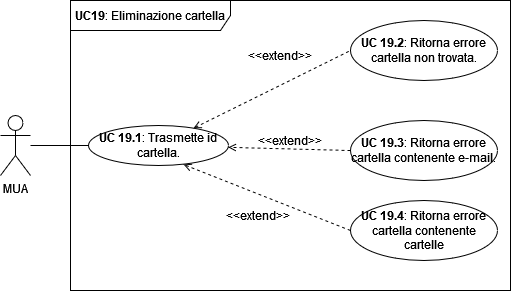
\includegraphics[width=0.85\textwidth]{sections/uc_imgs/UC19.png}
    \centering
    \caption{Diagramma sotto-casi UC 19}
\end{figure}

\subsubsection{UC 19.1 - Trasmette id cartella} \label{sec:UC19.1}
    \begin{itemize}
        \item \textbf{Attore principale}: MUA;
        \item \textbf{Descrizione}: il MUA invia l'id della cartella da eliminare al sistema;
        \item \textbf{Precondizioni}: il MUA sta usando la funzionalità di eliminazione di una cartella;
        \item \textbf{Postcondizioni}: il sistema elimina la cartella identificata dall'id fornito dal MUA;
        \item \textbf{Scenario principale}:
            \begin{enumerate}
                \item il MUA invia l'identificativo della cartella da eliminare al sistema;
                \item il sistema controlla che la cartella identificata rispetti i seguenti requisiti:
                \begin{itemize}
                    \item la cartella non contiene altre e-mail;
                    \item la cartella non contiene altre cartelle;
                \end{itemize}
            \end{enumerate}
        \item \textbf{Inclusioni}: nessuna;
        \item \textbf{Generalizzazioni}: nessuna;
        \item \textbf{Estensioni}:
            \begin{enumerate}[label=\alph*.]
                \item il sistema non riesce a eliminare la cartella perché non è stata trovata:
                \begin{enumerate}[label=\arabic*.]
                    \item il sistema ritorna un errore al MUA di cartella non trovata (\hyperref[sec:UC19.2]{UC 19.2}).
                \end{enumerate}
                \item il sistema non riesce a eliminare la cartella perché contiene delle e-mail:
                \begin{enumerate}[label=\arabic*.]
                    \item il sistema ritorna un errore al MUA di cartella contenente e-mail (\hyperref[sec:UC19.3]{UC 19.3}).
                \end{enumerate}
                \item il sistema non riesce a eliminare la cartella perché contiene altre cartelle:
                \begin{enumerate}[label=\arabic*.]
                    \item il sistema ritorna un errore al MUA di cartella contenente cartelle (\hyperref[sec:UC19.4]{UC 19.4}).
                \end{enumerate}
            \end{enumerate}
    \end{itemize}


\subsubsection{UC 19.2 - Ritorna errore cartella non trovata} \label{sec:UC19.2}
    \begin{itemize}
        \item \textbf{Attore principale}: MUA;
        \item \textbf{Descrizione}: il sistema non riesce a eliminare la cartella perché l'identificativo cartella non è stato trovato;
        \item \textbf{Precondizioni}: il MUA sta usando la funzionalità di invio id cartella al sistema di una cartella;
        \item \textbf{Postcondizioni}: il sistema non elimina la cartella, il MUA è stato notificato dell'errore;
        \item \textbf{Scenario principale}:
            \begin{enumerate}
                \item il sistema non trova la cartella con l'identificativo fornito dal MUA;
                \item il sistema non elimina la cartella e notifica il MUA dell'errore;
            \end{enumerate}
        \item \textbf{Inclusioni}: nessuna;
        \item \textbf{Generalizzazioni}: nessuna;
        \item \textbf{Estensioni}: nessuna.
    \end{itemize}
   
    \subsubsection{UC 19.3 - Ritorna errore cartella contenente e-mail} \label{sec:UC19.3}

    \begin{itemize}
        \item \textbf{Attore principale}: MUA;
        \item \textbf{Descrizione}: il sistema non riesce a eliminare la cartella perché una o più e-mail sono presenti all'interno di quella cartella;
        \item \textbf{Precondizioni}: il MUA sta usando la funzionalità di invio id di una cartella al sistema;
        \item \textbf{Postcondizioni}: il sistema non elimina la cartella, il MUA è stato notificato dell'errore;
        \item \textbf{Scenario principale}:
            \begin{enumerate}
                \item la cartella non soddisfa il requisito di non contenere e-mail;
                \item il sistema non elimina la cartella e notifica il MUA dell'errore;
            \end{enumerate}
        \item \textbf{Inclusioni}: nessuna;
        \item \textbf{Generalizzazioni}: nessuna;
        \item \textbf{Estensioni}: nessuna.
    \end{itemize}


    \subsubsection{UC 19.4 - Ricezione errore cartella contenente cartelle} \label{sec:UC19.4}

    \begin{itemize}
        \item \textbf{Attore principale}: MUA;
        \item \textbf{Descrizione}: il sistema non riesce a eliminare la cartella perché una o più cartelle sono presenti all'interno di quella cartella;
        \item \textbf{Precondizioni}: il MUA sta usando la funzionalità di invio id di una cartella al sistema;
        \item \textbf{Postcondizioni}: il sistema non elimina la cartella, il MUA è stato notificato dell'errore;
        \item \textbf{Scenario principale}:
            \begin{enumerate}
                \item la cartella non soddisfa il requisito di non contenere altre cartelle;
                \item il sistema non elimina la cartella e notifica il MUA dell'errore;
            \end{enumerate}
        \item \textbf{Inclusioni}: nessuna;
        \item \textbf{Generalizzazioni}: nessuna;
        \item \textbf{Estensioni}: nessuna.
    \end{itemize}

